\subsection{Sorted Data}
\subsubsection{Time}
Execution time unit: milliseconds

\begin{table}[h!]
\centering
\begin{tabular}{|l|r|r|r|r|r|r|}
\hline
\textbf{Algorithm} & \textbf{10000} & \textbf{30000} & \textbf{50000} & \textbf{100000} & \textbf{300000} & \textbf{500000} \\
\hline
Selection Sort & 83.5349 & 762.314 & 2093.73 & 8438.43 & 75874.9 & 210401 \\ \hline
Insertion Sort & 0.0043 & 0.013 & 0.0228 & 0.0452 & 0.1466 & 0.2558 \\ \hline
Shell Sort & 15.9199 & 166.915 & 454.441 & 1746.54 & 16108.9 & 72609.4 \\ \hline
Bubble Sort & 13.4474 & 123.507 & 329.481 & 1383.44 & 12187 & 34030.9 \\ \hline
Heap Sort & 0.691 & 2.2718 & 3.8386 & 8.0435 & 26.315 & 44.2006 \\ \hline
Merge Sort & 2.336 & 7.0626 & 11.8658 & 23.7198 & 73.8943 & 119.809 \\ \hline
Quick Sort & 78.4909 & 699.612 & 1986.74 & 7702.21 & 69509.3 & 198334 \\ \hline
Radix Sort & 0.1545 & 0.4646 & 0.943 & 1.5853 & 6.1696 & 10.6871 \\ \hline
Counting Sort & 0.016 & 0.0444 & 0.0809 & 0.208 & 0.7713 & 1.0371 \\ \hline
Binary Insertion Sort & 0.242 & 0.8476 & 1.3542 & 2.9678 & 10.6128 & 17.5126 \\ \hline
Shaker Sort & 0.0036 & 0.0094 & 0.0166 & 0.0418 & 0.1131 & 0.2715 \\ \hline
Flash Sort & 0.0948 & 0.2717 & 0.6822 & 1.1887 & 3.7231 & 5.9786 \\
\hline
\end{tabular}
\label{table:execution_time}
\end{table}

\begin{figure}[h]
    \centering
    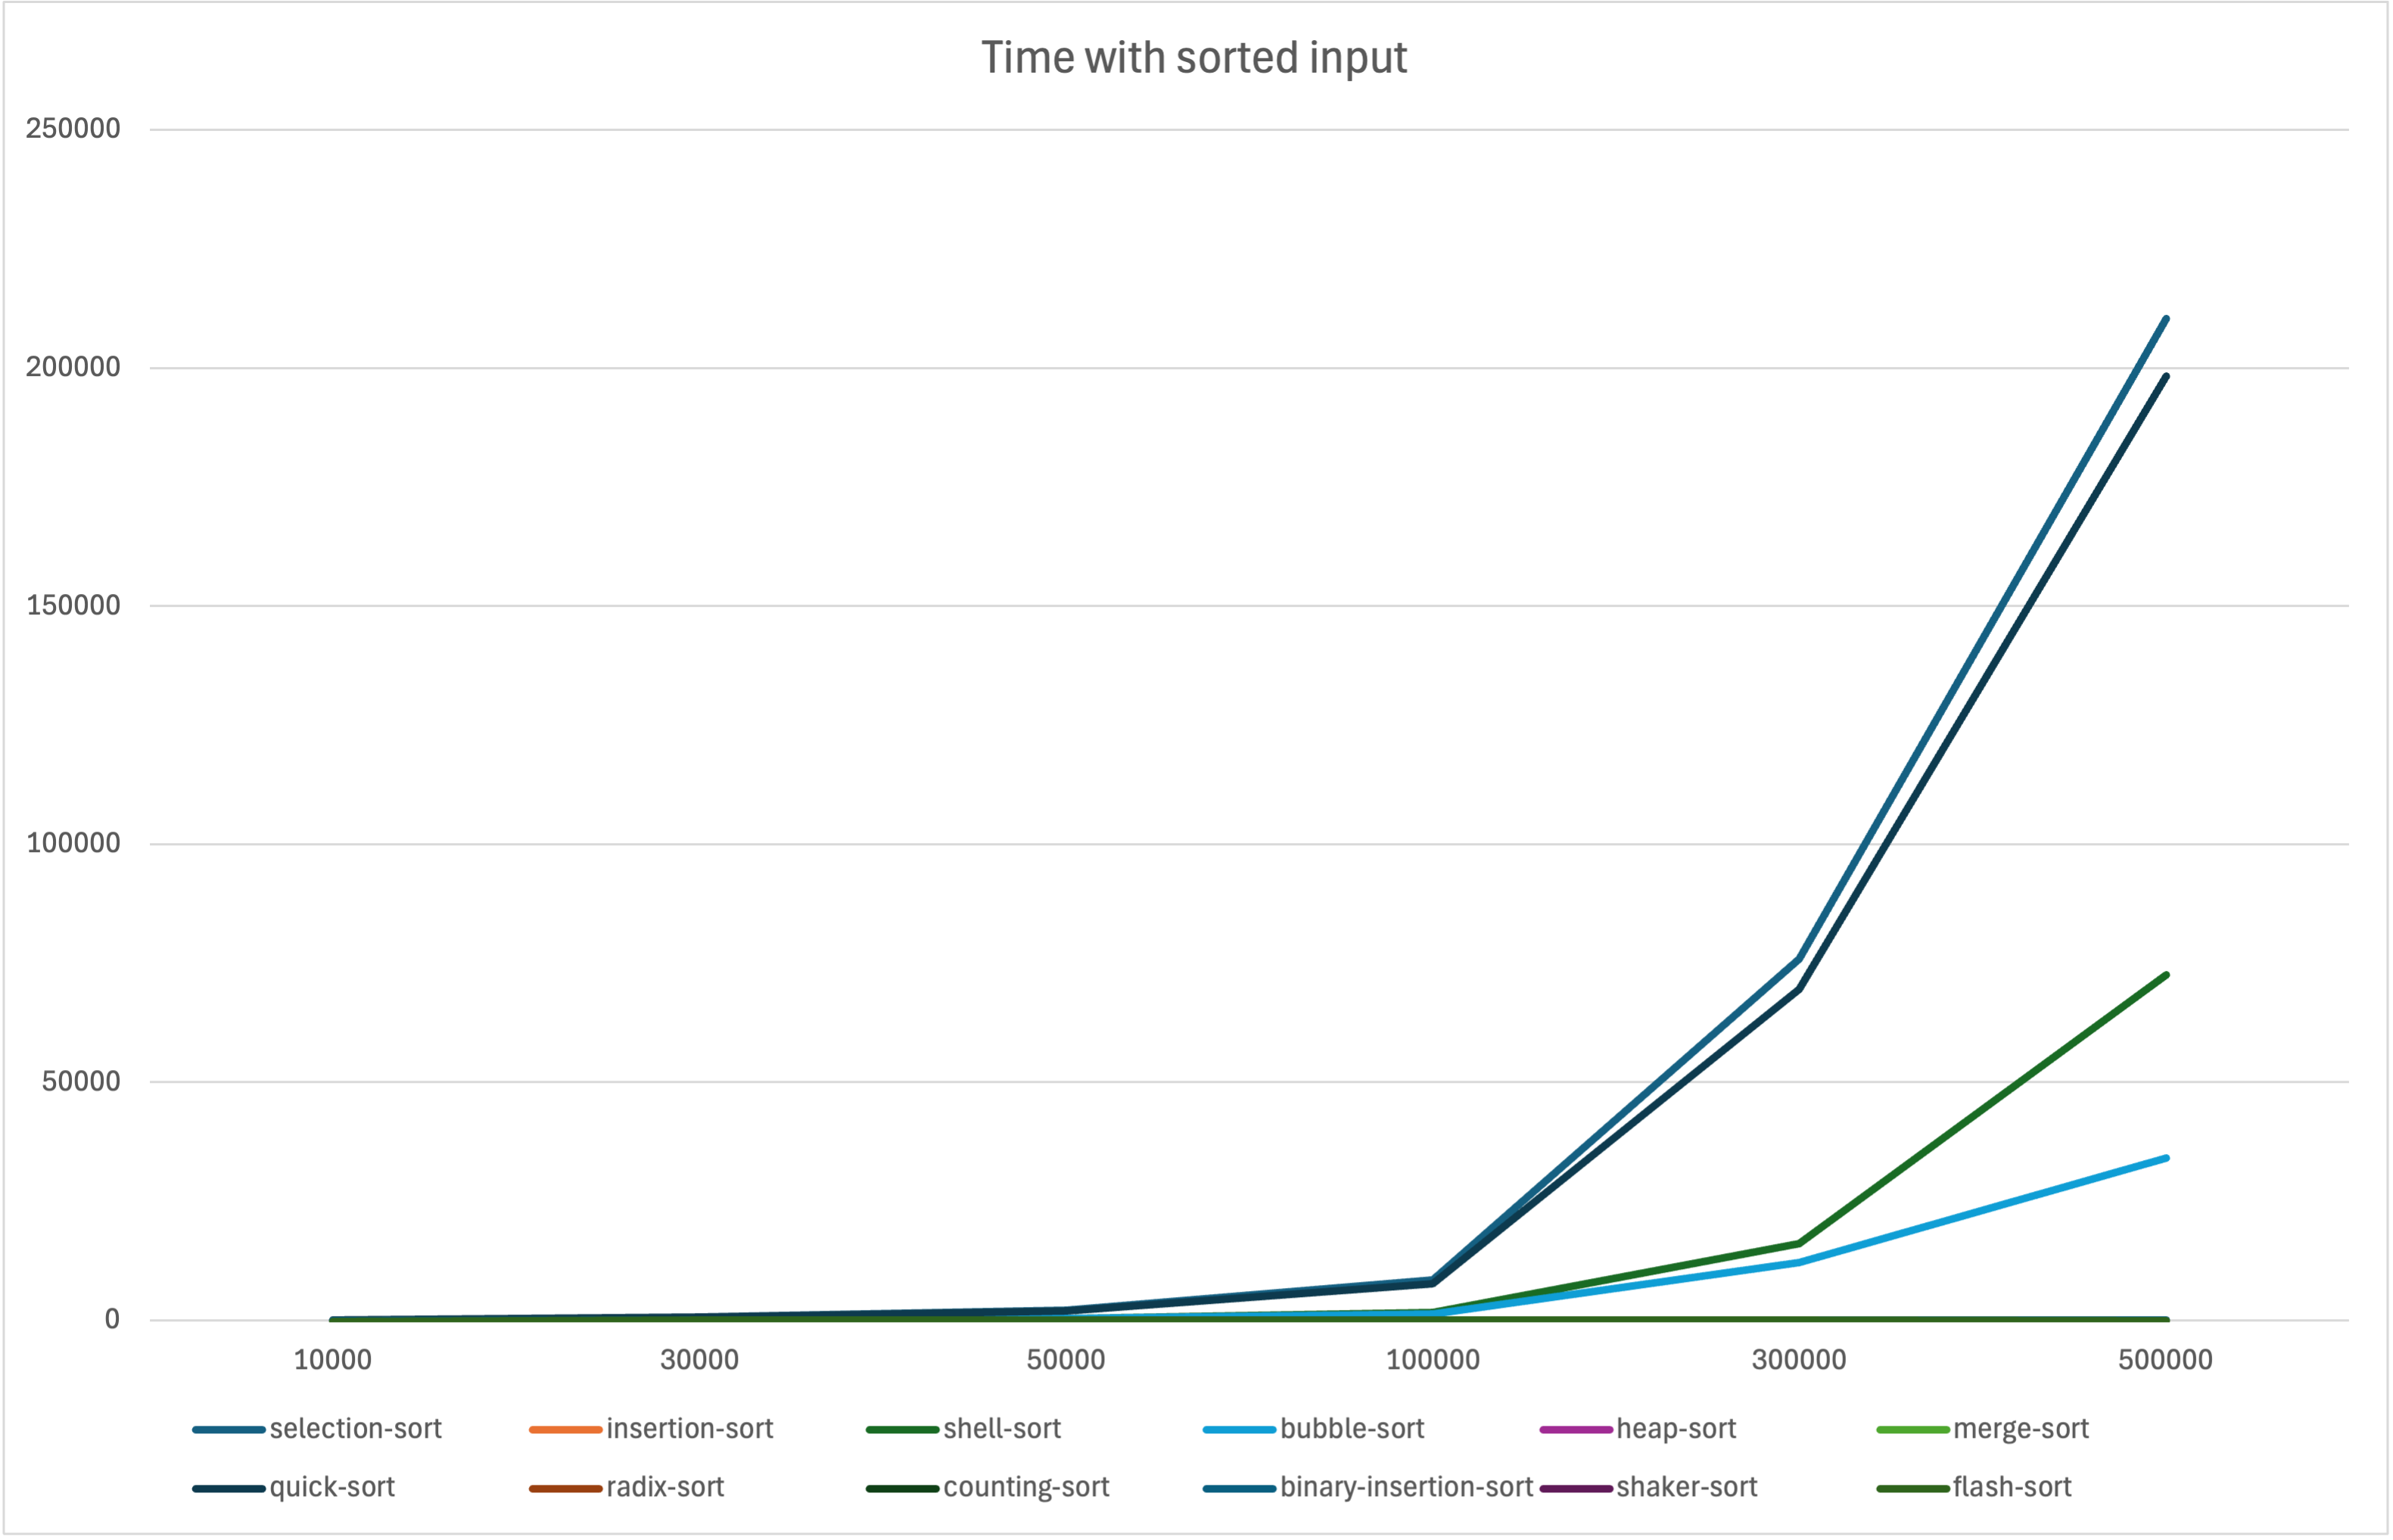
\includegraphics[scale=.65]{Figures/Visualization/Sorted_time.png}
    \caption{Execution time for Sorted data}
    \label{fig:enter-label}
\end{figure}

\textbf{Comments on the running time of sorting algorithms with sorted data}
\begin{enumerate}
    \item \textbf{Fastest Algorithms} \\
   - Insertion Sort: Extremely fast across all data sizes, maintaining very low execution times, which can be attributed to the sorted input allowing it to perform minimal operations. \\
   - Counting Sort and Radix Sort: Show low execution times, consistent with their linear or near-linear time complexity. \\
   - Flash Sort: Also performs well across different sizes, indicating efficiency in handling sorted data.

    \item \textbf{Slowest Algorithms} \\
   - Selection Sort: Performs poorly, with execution times increasing significantly with larger data sizes. This is due to its \(O(n^2)\) complexity. \\
   - Shell Sort and Bubble Sort: Have relatively high execution times, especially for larger data sizes, though they perform better than selection sort.

    \item \textbf{Moderate Performance} \\
   - Merge Sort, Heap Sort, Quick Sort: These algorithms show moderate execution times. Quick Sort's performance is likely impacted by pivot selection, which can lead to worse performance even on sorted input.
\end{enumerate}

\subsubsection{Comparison}

\vspace{5pt}

\begin{table}[h!]
\centering
\begin{tabular}{|l|r|r|r|r|r|r|}
\hline
\textbf{Algorithm} & \textbf{10000} & \textbf{30000} & \textbf{50000} & \textbf{100000} & \textbf{300000} & \textbf{500000} \\
\hline
Selection Sort & 100020001 & 900060001 & 2500100001 & 10000200001 & 90000600001 & 2.50001E+11 \\ \hline
Insertion Sort & 29998 & 89998 & 149998 & 299998 & 899998 & 1499998 \\ \hline
Shell Sort & 136486703 & 1228074234 & 3411144570 & 13643867417 & 1.2279E+11 & 3.41082E+11 \\ \hline
Bubble Sort & 100009999 & 900029999 & 2500049999 & 10000099999 & 90000299999 & 2.5E+11 \\ \hline
Heap Sort & 670329 & 2236648 & 3925351 & 8365080 & 27413230 & 47404886 \\ \hline
Merge Sort & 475242 & 1559914 & 2722826 & 5745658 & 18645946 & 32017850 \\ \hline
Quick Sort & 100019998 & 900059998 & 2500099998 & 10000199998 & 90000599998 & 2.50001E+11 \\ \hline
Radix Sort & 140051 & 510064 & 850064 & 1700064 & 6000077 & 10000777 \\ \hline
Counting Sort & 60003 & 180003 & 300003 & 600003 & 1800003 & 3000003 \\ \hline
Binary Insertion Sort & 370852 & 1251700 & 2203396 & 4706788 & 15527140 & 26927140 \\ \hline
Shaker Sort & 20002 & 60002 & 100002 & 200002 & 600002 & 1000002 \\ \hline
Flash Sort & 119000 & 357000 & 595000 & 1190000 & 3570000 & 5950000 \\
\hline
\end{tabular}
\label{table:number_of_comparisons}
\end{table}

\textbf{Comments on the number of comparisons of sorting algorithms with sorted data}
\begin{enumerate}
    \item \textbf{Fewest Comparisons} \\
   - Counting Sort: Performs the fewest comparisons as it is a non-comparison-based sort. \\
   - Insertion Sort: Very few comparisons are needed due to the already sorted input, similar to its execution time performance. \\
   - Flash Sort: Also shows low comparisons, consistent with its efficient performance.

    \item \textbf{Most Comparisons} \\
   - Shell Sort: Has an extremely high number of comparisons, especially at larger data sizes. \\
   - Bubble Sort: Also shows a high number of comparisons, though not as much as shell sort. \\
   - Selection Sort and Quick Sort: Both have high numbers of comparisons due to their \(O(n^2)\) and \(O(n\log n)\) complexities, respectively.
\end{enumerate}

\begin{figure}[h]
    \centering
    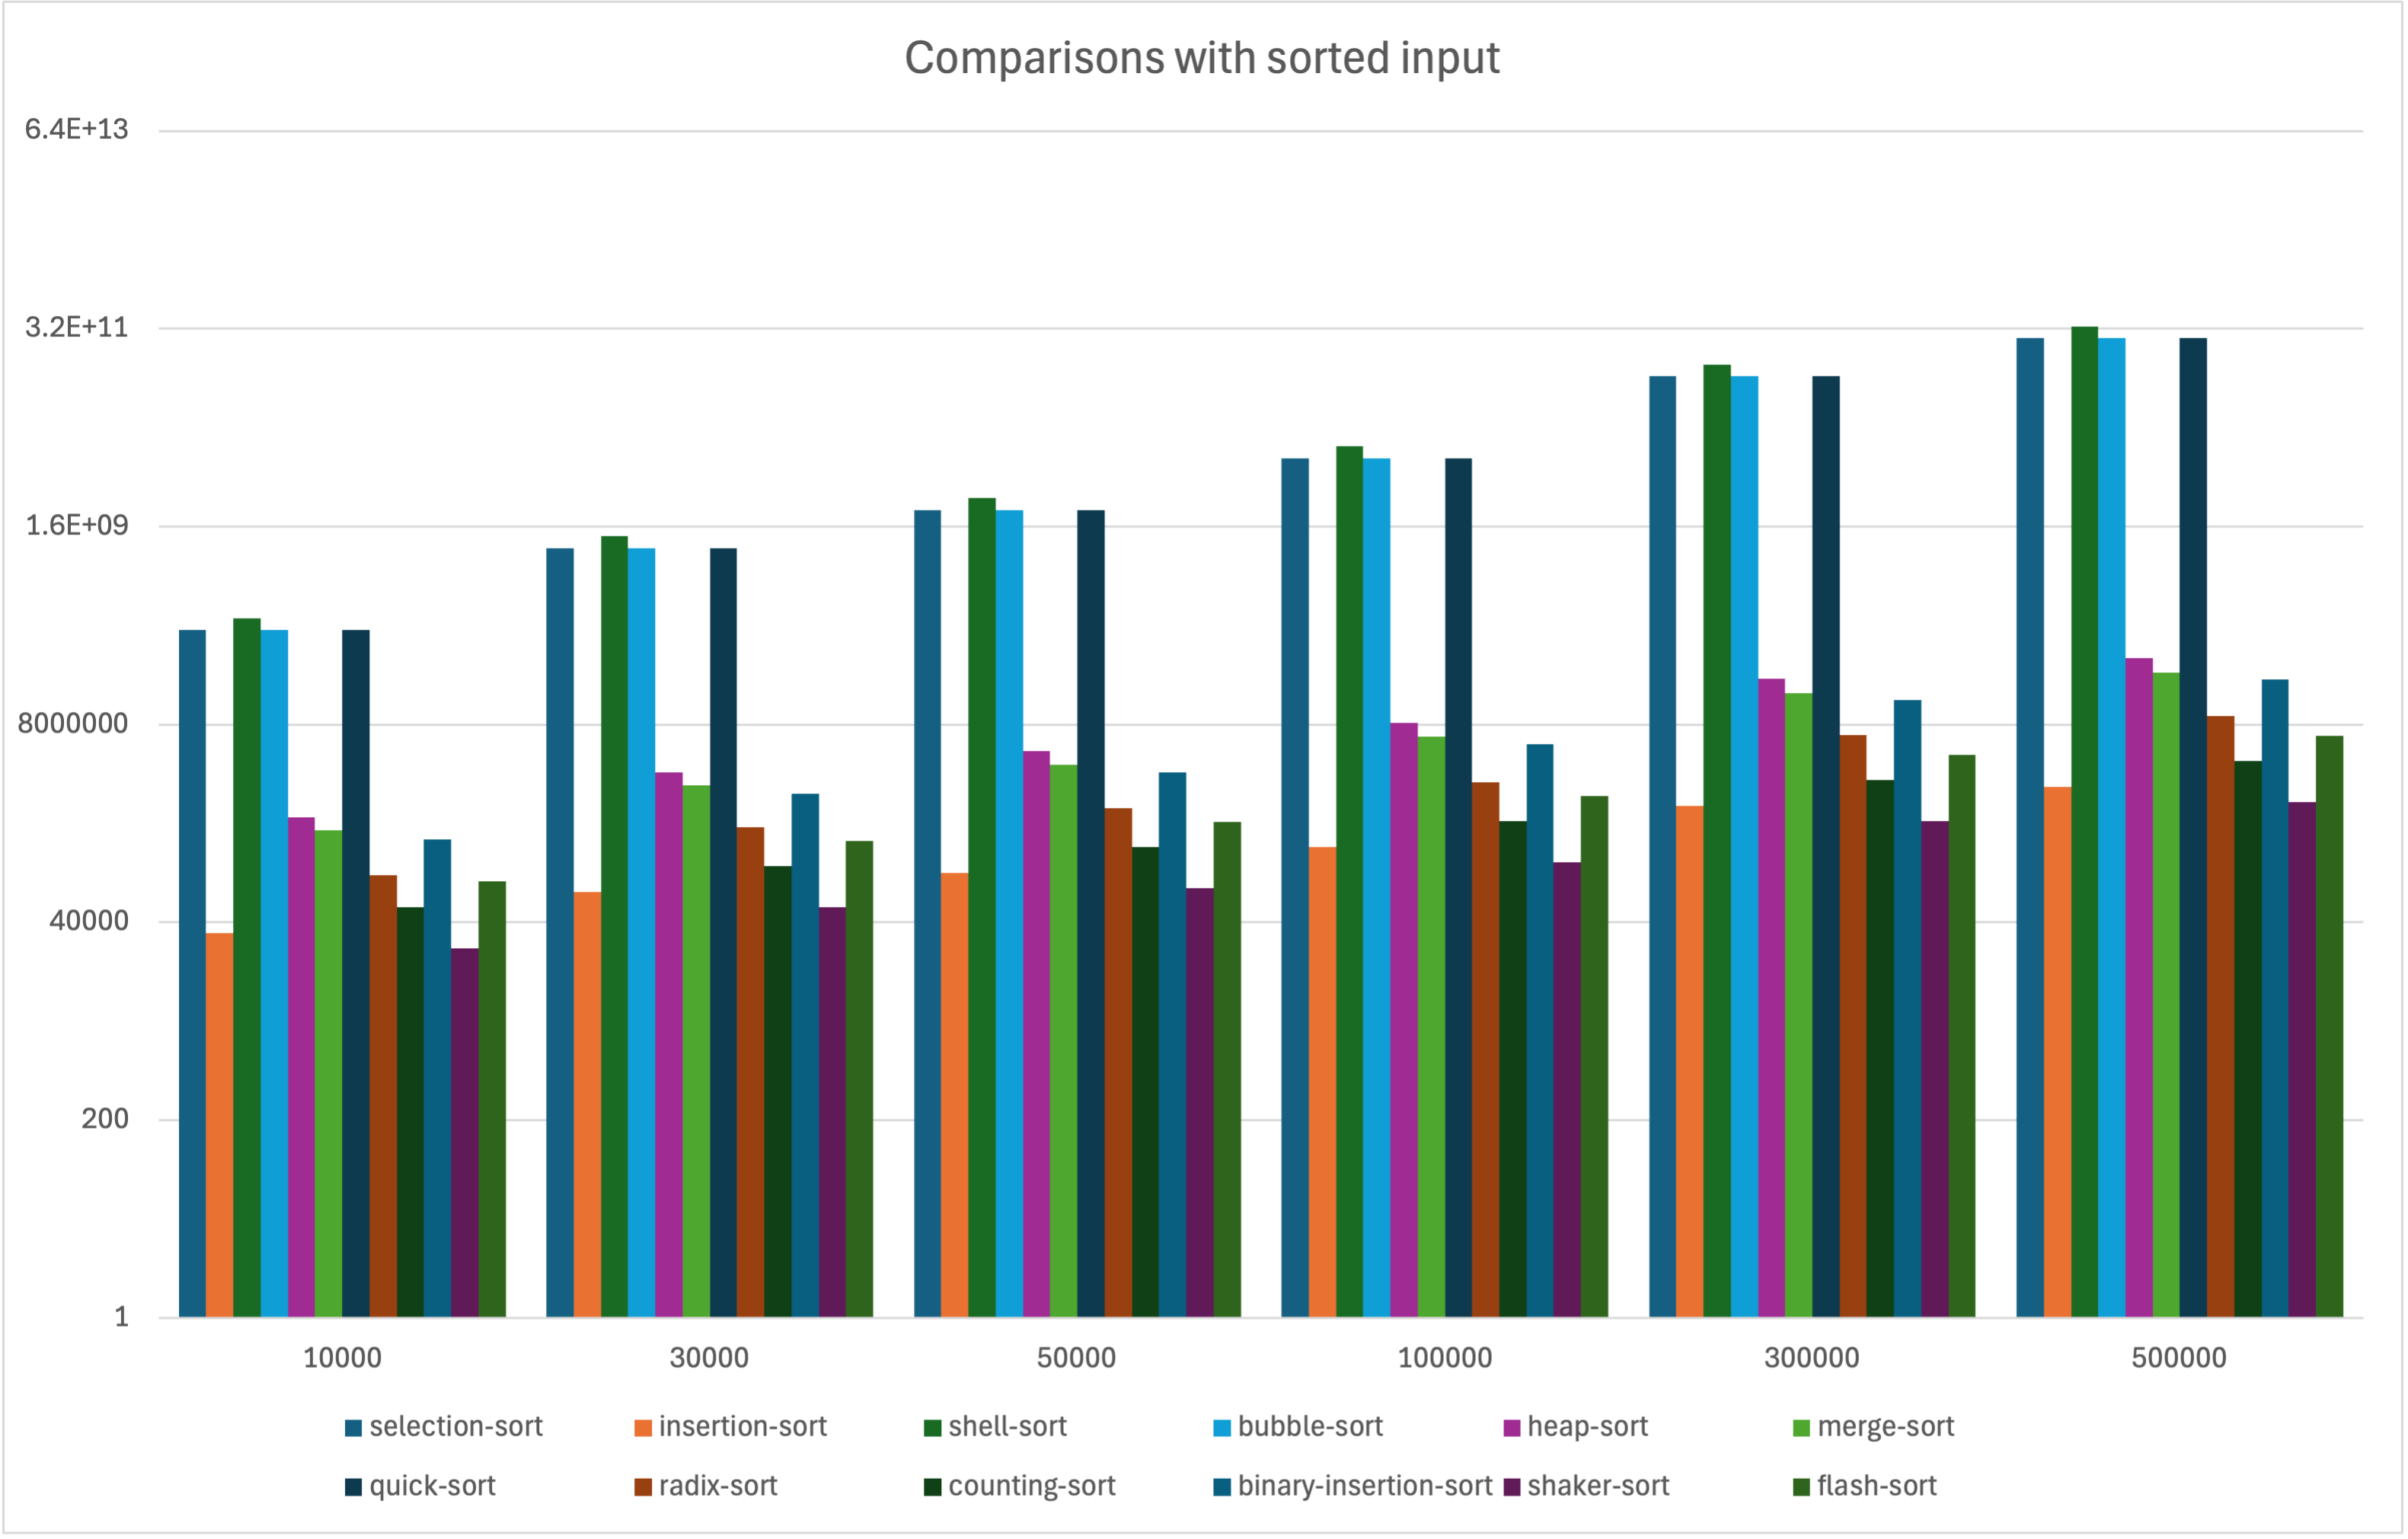
\includegraphics[scale=.65]{Figures/Visualization/Sorted_compare.png}
    \caption{Number of comparisons of the algorithm for Sorted data}
    \label{fig:enter-label}
\end{figure}

\newpage

\subsubsection{Overall}
\textbf{Overall comments on algorithms based on all data and size}
\begin{enumerate}
    \item \textbf{Data Order and Data Size} \\
   - For sorted data, insertion sort, counting sort, and flash sort are the best performers in terms of execution time and number of comparisons. \\
   - Selection sort, shell sort, and bubble sort are consistently the slowest and have the highest number of comparisons. \\
   - Merge sort, heap sort, and quick sort offer a balance but do not outperform the linear or near-linear algorithms for sorted data.

    \item \textbf{Stability:} \\
   - Stable Algorithms: Insertion sort, merge sort, and bubble sort are stable sorting algorithms. Insertion sort performs the best with sorted input among the stable sorts. \\
   - Unstable Algorithms: Quick sort, heap sort, and shell sort are unstable. Despite quick sort and heap sort being faster than shell sort in most cases, they are still outperformed by the linear time algorithms on sorted data.
\end{enumerate}

